% Created 2022-06-27 Mon 10:03
% Intended LaTeX compiler: pdflatex
\documentclass[presentation,aspectratio=169]{beamer}
\usepackage[utf8]{inputenc}
\usepackage[T1]{fontenc}
\usepackage{graphicx}
\usepackage{grffile}
\usepackage{longtable}
\usepackage{wrapfig}
\usepackage{rotating}
\usepackage[normalem]{ulem}
\usepackage{amsmath}
\usepackage{textcomp}
\usepackage{amssymb}
\usepackage{capt-of}
\usepackage{hyperref}
\usepackage{khpreamble}
\DeclareMathOperator{\atantwo}{atan2}
\usetheme{default}
\author{Kjartan Halvorsen}
\date{2022-06-28}
\title{Frequency response}
\hypersetup{
 pdfauthor={Kjartan Halvorsen},
 pdftitle={Frequency response},
 pdfkeywords={},
 pdfsubject={},
 pdfcreator={Emacs 26.3 (Org mode 9.4.6)}, 
 pdflang={English}}
\begin{document}

\maketitle

\section{Bode diagram}
\label{sec:org12b14cf}

\begin{frame}[label={sec:orge6079e2}]{Response of LTI systems to sinusoids}
\begin{center}
  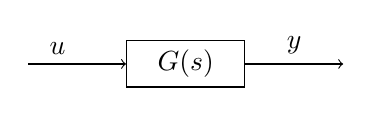
\begin{tikzpicture}[scale = 0.8, node distance=20mm, block/.style={rectangle, draw, minimum width=15mm}, sumnode/.style={circle, draw, inner sep=2pt}]

  \node[coordinate] (refinput) {};
  \node[block, right of=refinput] (motor) {$G(s)$};
  \node[coordinate, right of=motor, node distance=20mm] (output) {};

  \draw[->] (refinput) -- node[above, pos=0.3] (voltsignal) {$u$} (motor);
  \draw[->] (motor) -- node[above, pos=0.5] (velsignal) {$y$} (output);
  \end{tikzpicture}
\end{center}

Let \(u(t) = \sin\omega_1 t\). Then, after transients have died out,
\[ y(t) = |G(i\omega_1)| \sin \big( \omega_1 t + \arg G(i\omega_1)\big). \]
\end{frame}


\begin{frame}[label={sec:org2462e6a}]{The Bode diagram}
\[ y(t) = \underbrace{|G(i\omega_1)|}_{\text{amplification}} \sin \big( \omega_1 t + \underbrace{\arg G(i\omega_1)}_{\text{phase shift}} \big) \]

The Bode diagram shows the magnitude and phase of the transfer function evaluated on the positive imaginary axis. It thus contains all information about the steady-state response of the system to input signals of different frequency.
\end{frame}


\begin{frame}[label={sec:orgade3c46}]{Specifications on the frequency properties of the closed-loop system}
\begin{center}
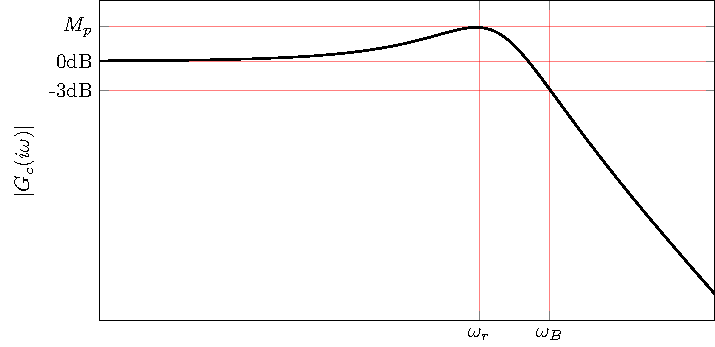
\includegraphics[width=0.899\linewidth]{../../figures/spec-bode-closed-loop-new}
\end{center}
\end{frame}

\begin{frame}[label={sec:orgd748c93}]{Exercise: Reading the Bode diagram}
\begin{center}
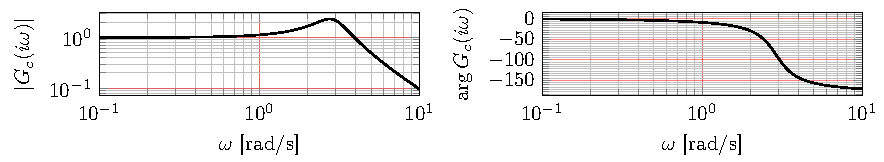
\includegraphics[width=\linewidth]{../../figures/alias-example-bode-GC}
\end{center}
which of the below frequency responses \alert{is not} compatible with the Bode diagram?

\begin{center}
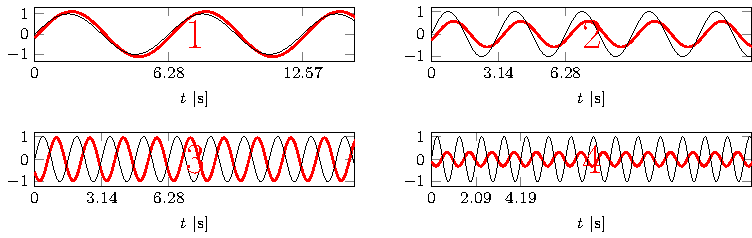
\includegraphics[width=\linewidth]{../../figures/alias-example-bode-timeseries}
\end{center}
\end{frame}

\begin{frame}[label={sec:org47b536e}]{Stability of the closed-loop system}
 \begin{center}
 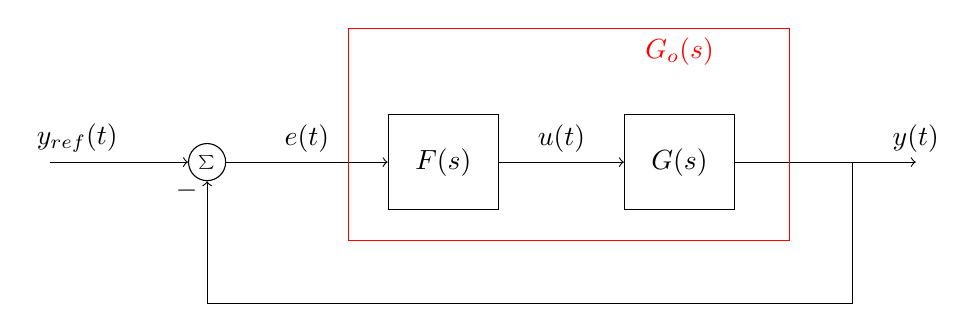
\begin{tikzpicture}
\tikzset{node distance=2cm, 
    block/.style={rectangle, draw, minimum height=12mm, minimum width=14mm},
    sumnode/.style={circle, draw, inner sep=2pt}        
}

  \node[coordinate] (input) {};
  \node[sumnode, right of=input, node distance=20mm] (sum) {\tiny $\sum$};
  \node[block,right of=sum, node distance=30mm] (fb) {$F(s)$};
  \node[block,right of=fb, node distance=30mm] (plant) {$G(s)$};
  \node[coordinate, right of=plant, node distance=30mm] (output) {};
  \node[coordinate, right of=plant, node distance=22mm] (measure) {};
  \draw[->] (input) -- node[above, pos=0.2] {$y_{ref}(t)$} (sum);
  \draw[->] (sum) -- node[above] {$e(t)$} (fb);
  \draw[->] (fb) -- node[above] {$u(t)$} (plant);
  \draw[->] (plant) -- node[at end, above] {$y(t)$} (output);
  \draw[->] (measure) -- ++(0, -18mm) -| (sum) node[left, pos=0.96] {$-$};
  \draw[red] (3.8, -1) rectangle (9.4, 1.7);
  \node[red] at (8, 1.4) {$G_o(s)$};
  \end{tikzpicture}
\end{center}
\end{frame}

\begin{frame}[label={sec:orgd22ccdc}]{Stability of the closed-loop system}
 \begin{center}
 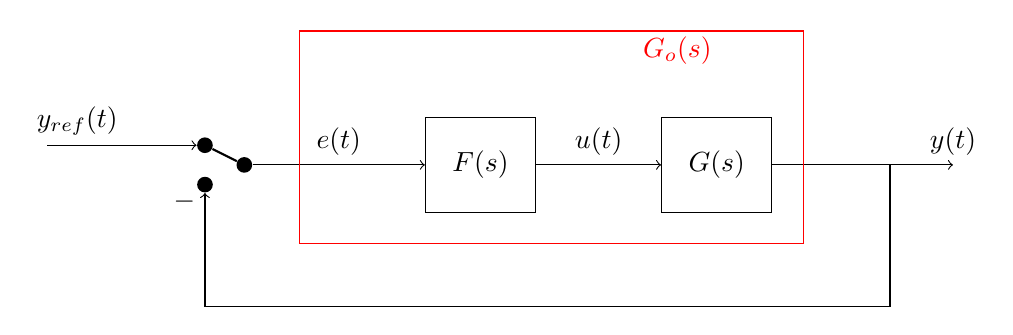
\begin{tikzpicture}
\tikzset{node distance=2cm, 
    block/.style={rectangle, draw, minimum height=12mm, minimum width=14mm},
    sumnode/.style={circle, draw, inner sep=2pt}        
}

  \node[coordinate] (input) {};
  \node[circle, black, fill, inner sep=2pt, right of=input, node distance=20mm] (sum) {};
  \node[circle, black, fill, inner sep=2pt, below of=sum, node distance=5mm] (sum2) {};
  \node[coordinate, right of=sum, node distance=5mm] (sum3) {};
  \node[circle, black, fill, inner sep=2pt, below of=sum3, node distance=2.5mm] (sum4) {};
  \node[block,right of=sum4, node distance=30mm] (fb) {$F(s)$};
  \node[block,right of=fb, node distance=30mm] (plant) {$G(s)$};
  \node[coordinate, right of=plant, node distance=30mm] (output) {};
  \node[coordinate, right of=plant, node distance=22mm] (measure) {};
  \draw[->] (input) -- node[above, pos=0.2] {$y_{ref}(t)$} (sum);
  \draw[->] (sum4) -- node[above] {$e(t)$} (fb);
  \draw[->] (fb) -- node[above] {$u(t)$} (plant);
  \draw[->] (plant) -- node[at end, above] {$y(t)$} (output);
  \draw[->] (measure) -- ++(0, -18mm) -| (sum2) node[left, pos=0.96] {$-$};
  \draw[red] (3.2, -1.25) rectangle (9.6, 1.45);
  \node[red] at (8, 1.2) {$G_o(s)$};
  \draw[thick] (sum) to (sum4);
  \end{tikzpicture}
\end{center}

\begin{center}

  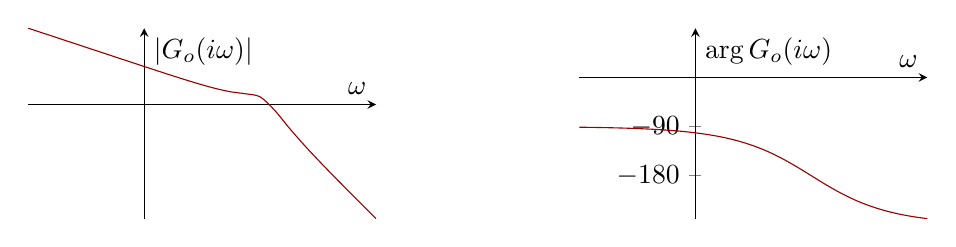
\begin{tikzpicture}
    \begin{semilogxaxis}[%
      width=6cm,
      height=4cm,
      axis lines=center,
      xtick = {1},
      xticklabels = {$\omega_1$},
      ytick = \empty,
      ylabel = {$|G_o(i\omega)|$},
      xlabel = {$\omega$},
      ]
      \addplot[solid, red!60!black, smooth, domain=0.1:100] {20*log10(10/x * 100/(sqrt(pow((100-x*x),2) + 20*20*x)))};
    \end{semilogxaxis}

    \begin{semilogxaxis}[%
    xshift=7cm,
    width=6cm,
      height=4cm,
      axis lines=center,
      xtick = {1},
      xticklabels = {$\omega_1$},
      ytick = {0,-90,-180, -270},
      ylabel = {$\arg G_o(i\omega)$},
      xlabel = {$\omega$},
      ymax = 90,
      ]
      \addplot[solid, red!60!black, smooth, domain=0.1:100] {-90 - atan2(20*x, 100-x*x)};
    \end{semilogxaxis}

    \end{tikzpicture}
\end{center}
\end{frame}


\begin{frame}[label={sec:orgcc54f31}]{From loop gain to closed-loop gain}
 \begin{center}
 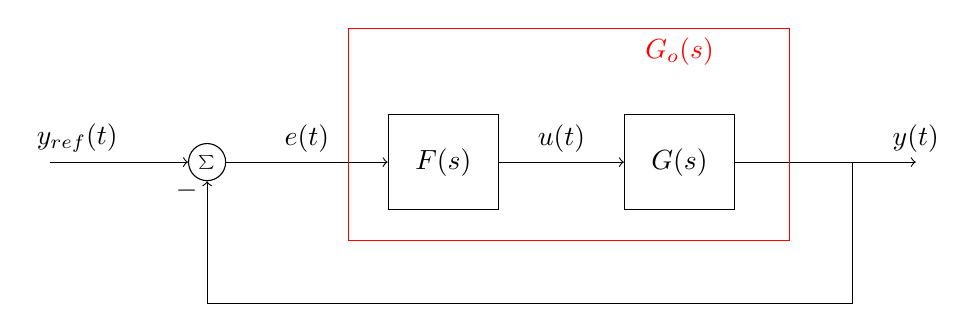
\begin{tikzpicture}
\tikzset{node distance=2cm, 
    block/.style={rectangle, draw, minimum height=12mm, minimum width=14mm},
    sumnode/.style={circle, draw, inner sep=2pt}        
}

  \node[coordinate] (input) {};
  \node[sumnode, right of=input, node distance=20mm] (sum) {\tiny $\sum$};
  \node[block,right of=sum, node distance=30mm] (fb) {$F(s)$};
  \node[block,right of=fb, node distance=30mm] (plant) {$G(s)$};
  \node[coordinate, right of=plant, node distance=30mm] (output) {};
  \node[coordinate, right of=plant, node distance=22mm] (measure) {};
  \draw[->] (input) -- node[above, pos=0.2] {$y_{ref}(t)$} (sum);
  \draw[->] (sum) -- node[above] {$e(t)$} (fb);
  \draw[->] (fb) -- node[above] {$u(t)$} (plant);
  \draw[->] (plant) -- node[at end, above] {$y(t)$} (output);
  \draw[->] (measure) -- ++(0, -18mm) -| (sum) node[left, pos=0.96] {$-$};
  \draw[red] (3.8, -1) rectangle (9.4, 1.7);
  \node[red] at (8, 1.4) {$G_o(s)$};
  \end{tikzpicture}
\end{center}

\pause
\[ G_c(i\omega) = \frac{G(i\omega)F(i\omega)}{1 + G(i\omega)F(i\omega)} = \frac{G_o(i\omega)}{1 + G_o(i\omega)} \]
\pause
\[ |G_c(i\omega)| = \frac{|G_o(i\omega)|}{|1 + G_o(i\omega)|} = \frac{|G_o(i\omega)|}{|G_o(i\omega) - (-1)|} \]

\pause
\alert{Keep the loop gain \(G_o(i\omega)\) away from -1!} 
\end{frame}
\end{document}